\subsection{SMR的dataflow}
\subsection{流水线并行}
%主要讲述流水线并行的优势,以及各个部件,上层能够看到的,下一章再来详细介绍底层实现上的支持
如上问所述,影响Phoenix性能的关键因素是
barrier的存在,
以及Posix线程库较差的scalability。
DMR基于一种新的Producer-Consumer模型,
打破barrier,且不再使用线程库,
从而提高处理的效率和scalability。
本节阐述新的Producer-Consumer的设计原理,
DMR的流水并行,以及地址空间的隔离。

多核下的MapReduce模型中,
Map阶段产生的key-value,都存放于一个共享的中间结构,
之前的很多研究都显示,
影响多核MapReduce系统性能的关键因素是
对该中间结构的操作效率\cite{mao2010metis}。
\begin{figure}[!h!t]  
    \centering
    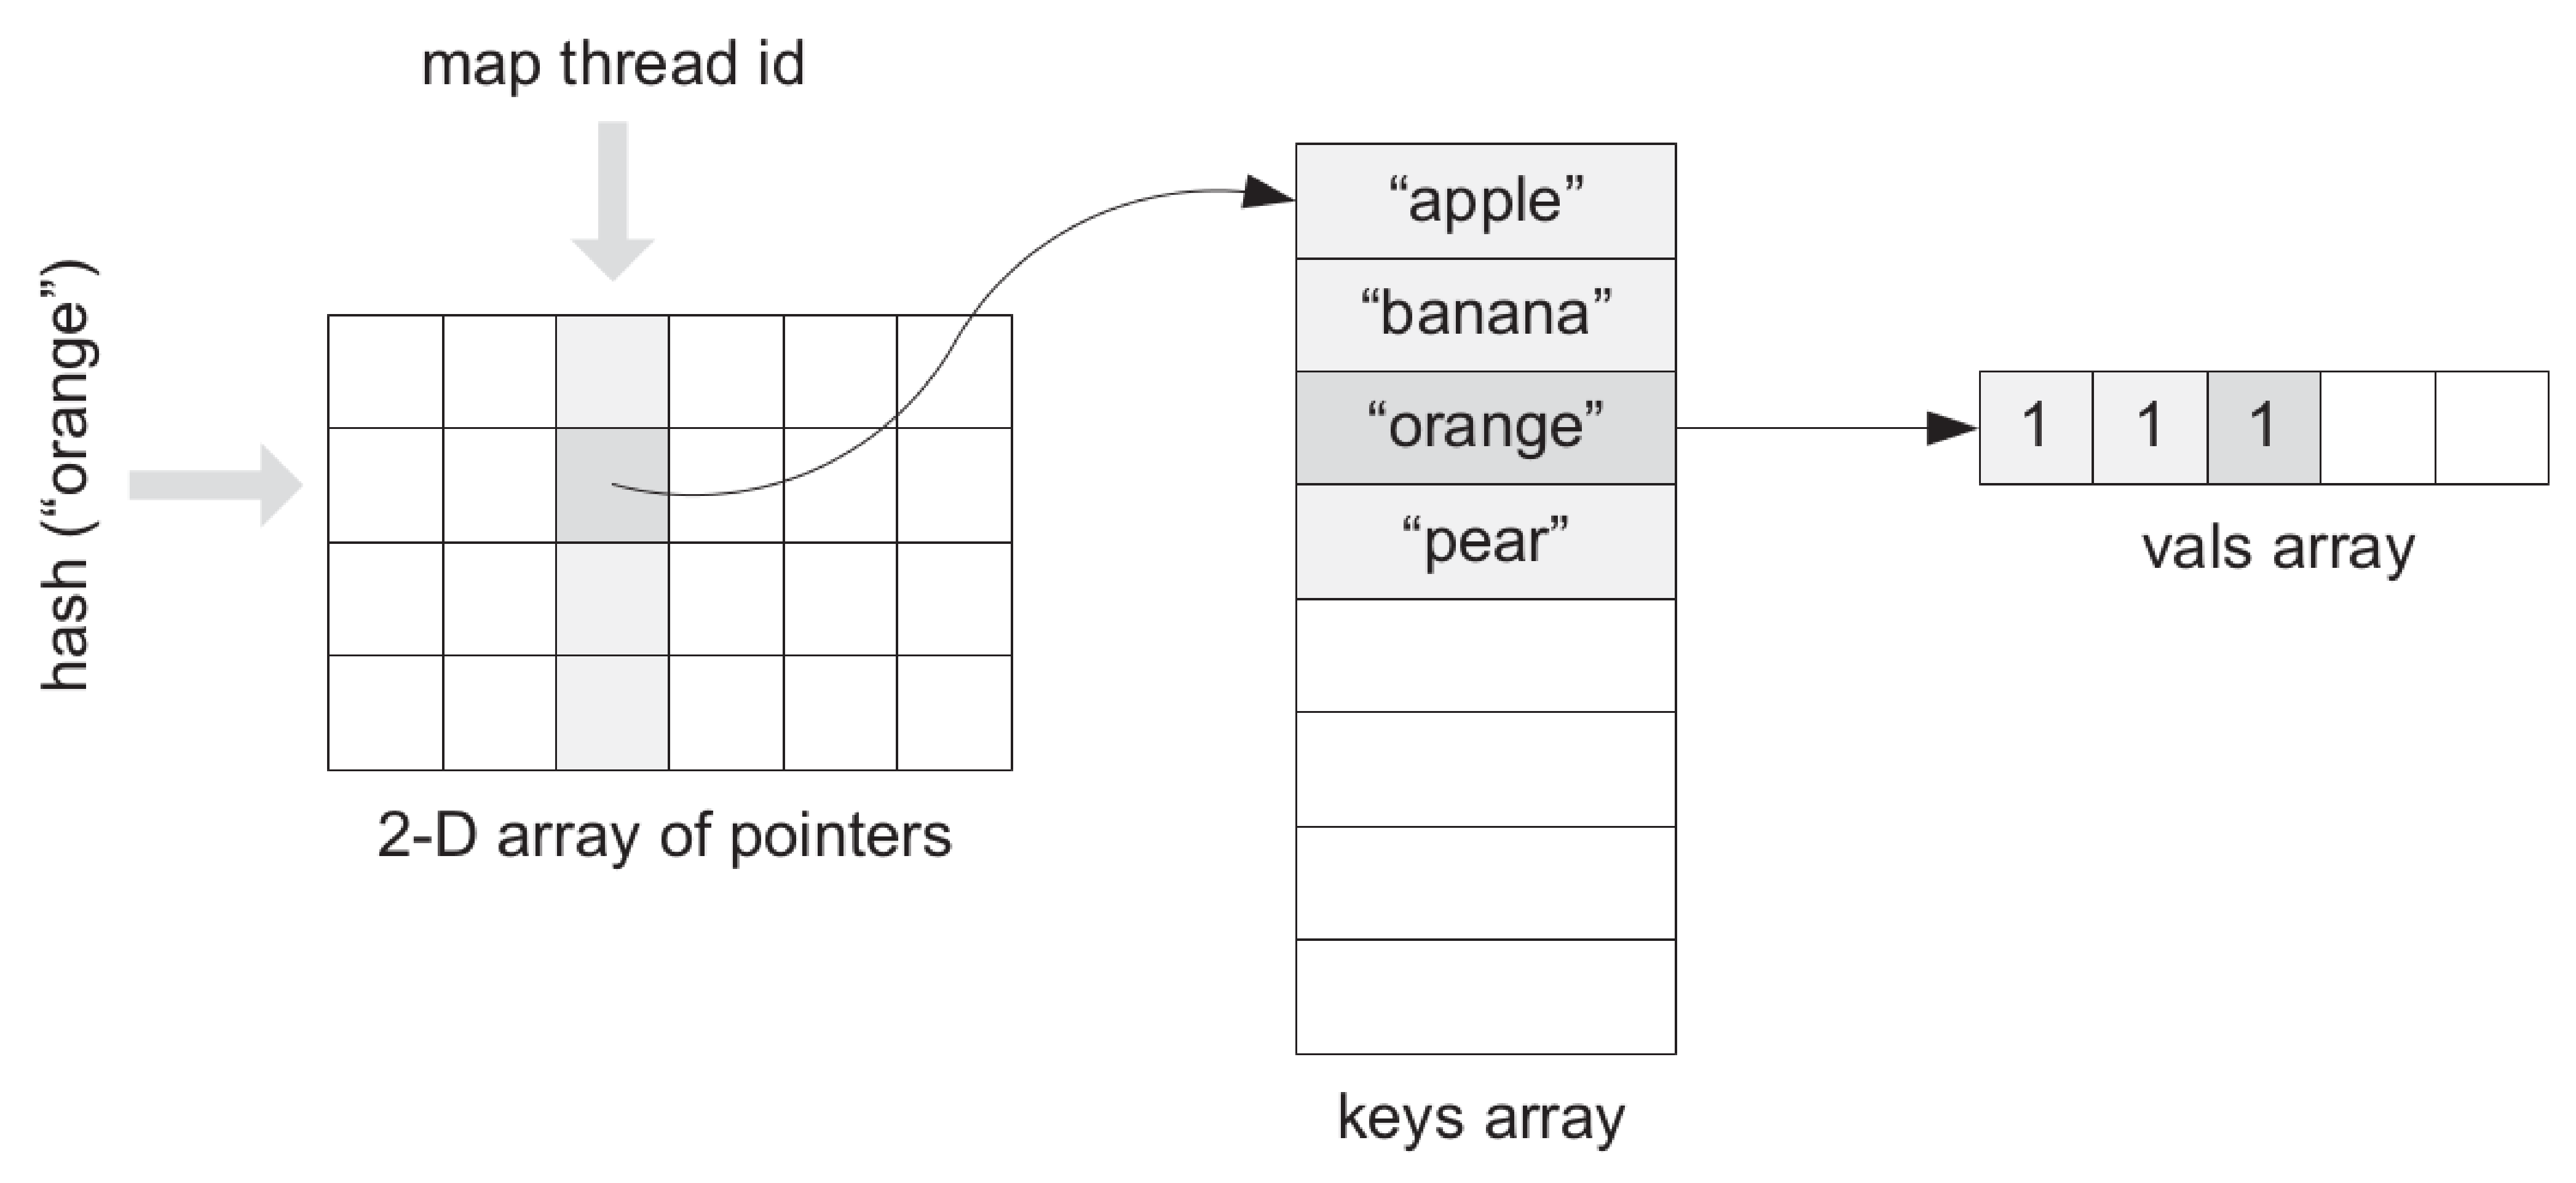
\includegraphics[width=0.75\textwidth]{img/phoenix_intermediate.eps}
    \caption{phoenix intermediate is a gobal array}
    \label{phoenix:intermediate}
\end{figure}

Phoenix中间结构是一个全局的二维数组
(如图\ref{phoenix:intermediate}),
为了避免多个map worker和reduce worker对
共享的中间结构竞争,
Phoenix采用两种策略:
\begin{itemize}
  \item 对全局的二维数组进行划分:
  每个map操作每一行,每个reduce操作每一列。
  即map和reduce都拥有自己独立的读写区域。
  可有效避免多个map或多个reduce之间读写同一区域的竞争。
  
  \item 为了避免map和reduce的交织,
  Phoenix在map和reduce之间加入barrier,
  即Map阶段结束后,才能开始Reduce阶段。
  可以避免map和reduce对同一区域的竞争。
\end{itemize}

Map阶段通常会进行大量的计算,
Reduce阶段则是需要大量的内存访问。
如果像Phoenix一样,在Map和Reduce之间加入barrier,
即等到所有的Map阶段结束,才开始reduce计算,
就会存在两个问题:
\begin{itemize}
  \item 不利于CPU的利用率,Map阶段会集中使用CPU,
  而Reduce阶段需要大量的内存访问,
  CPU资源被浪费。
  \item reduce阶段开始时间,由最慢的map worker决定;
  当某个map worker非常慢,便会影响整体的性能
\end{itemize}

DMR设计实现中,首先打破Phoenix的barrier,
不再使用共享的中间结构,DMR中的每个map worker
都拥有属于自己的私有buffer(buffer的设计细节见下一节),
一旦buffer中的key-value达到一定的阈值便发送给相应的reduce worker,
reduce收到key-value后,不等map worker结束便开始reduce工作,
即Map和Reduce阶段并发的粒度变小,
这既能充分利用资源,又能提高计算的速度。

特别地,当我们采用array buffer,
并且在map阶段不开启combiner时,
Map阶段不需要对key-value排序,即无需key的查找和插入,以及memmove等操作。
map worker产生key-value后,只需简单地将其追加到buffer中即可,
这减轻的Map阶段的工作量。key-value的排序工作由Reduce承担,
reduce worker对收到的key-value进行有序插入。
虽然整个过程的工作量并未减少,
但是Reduce的排序工作与Map阶段是并发执行的,
从而整个过程的时间变小,提高运行的效率。

此外,为了防止数据的倾斜,即大量的key-value被发送到一个reduce worker,
在Reduce阶段,我们添加了局部的reduce过程(即combiner),
一旦某个Reduce收到某个key-value的数量超过预先设定的值,
便会触发combiner,从而避免过多的内存分配带来的开销,
防止内存溢出。

DMR中map worker和reduce worker之所以能够进行流水并行执行,
是因为它们基于一个Producer-Consumer model,
在这个model中,每个map worker都拥有一个私有的buffer,
map woker是这个buffer的生产者,reduce是buffer的消费者,
当buffer中的数据达到一个阈值时,
reduce便可以取到buffer中的数据开始工作,
而不需要等到所有map结束。



\subsubsection{produce-consume模型}
%将详细介绍这个producer-consumer模型的所有特点,
如上所述,map worker和reducer worker的流水执行,
需要底层Producer-Consumer模型的支持,
本节将详细描述该模型的设计原理。

通常producer-consumer模型中,
producer和consumer之间有一个queue,
producer向queue中添加任务,
consumer从queue中读取任务。
MRPhi\cite{lu2013mrphi}为了使Map和Reduce并行执行,
便是采用这种Producer-Consumer模型,
具体如图\ref{mrphi:pc-model}所示。
在这个模型中,每个reduce worker对应一个queue,
map worker产生的数据会追加到queue中,
这是一个多对一的produce-consume模型,
\begin{figure}[!h!t]  
    \centering
    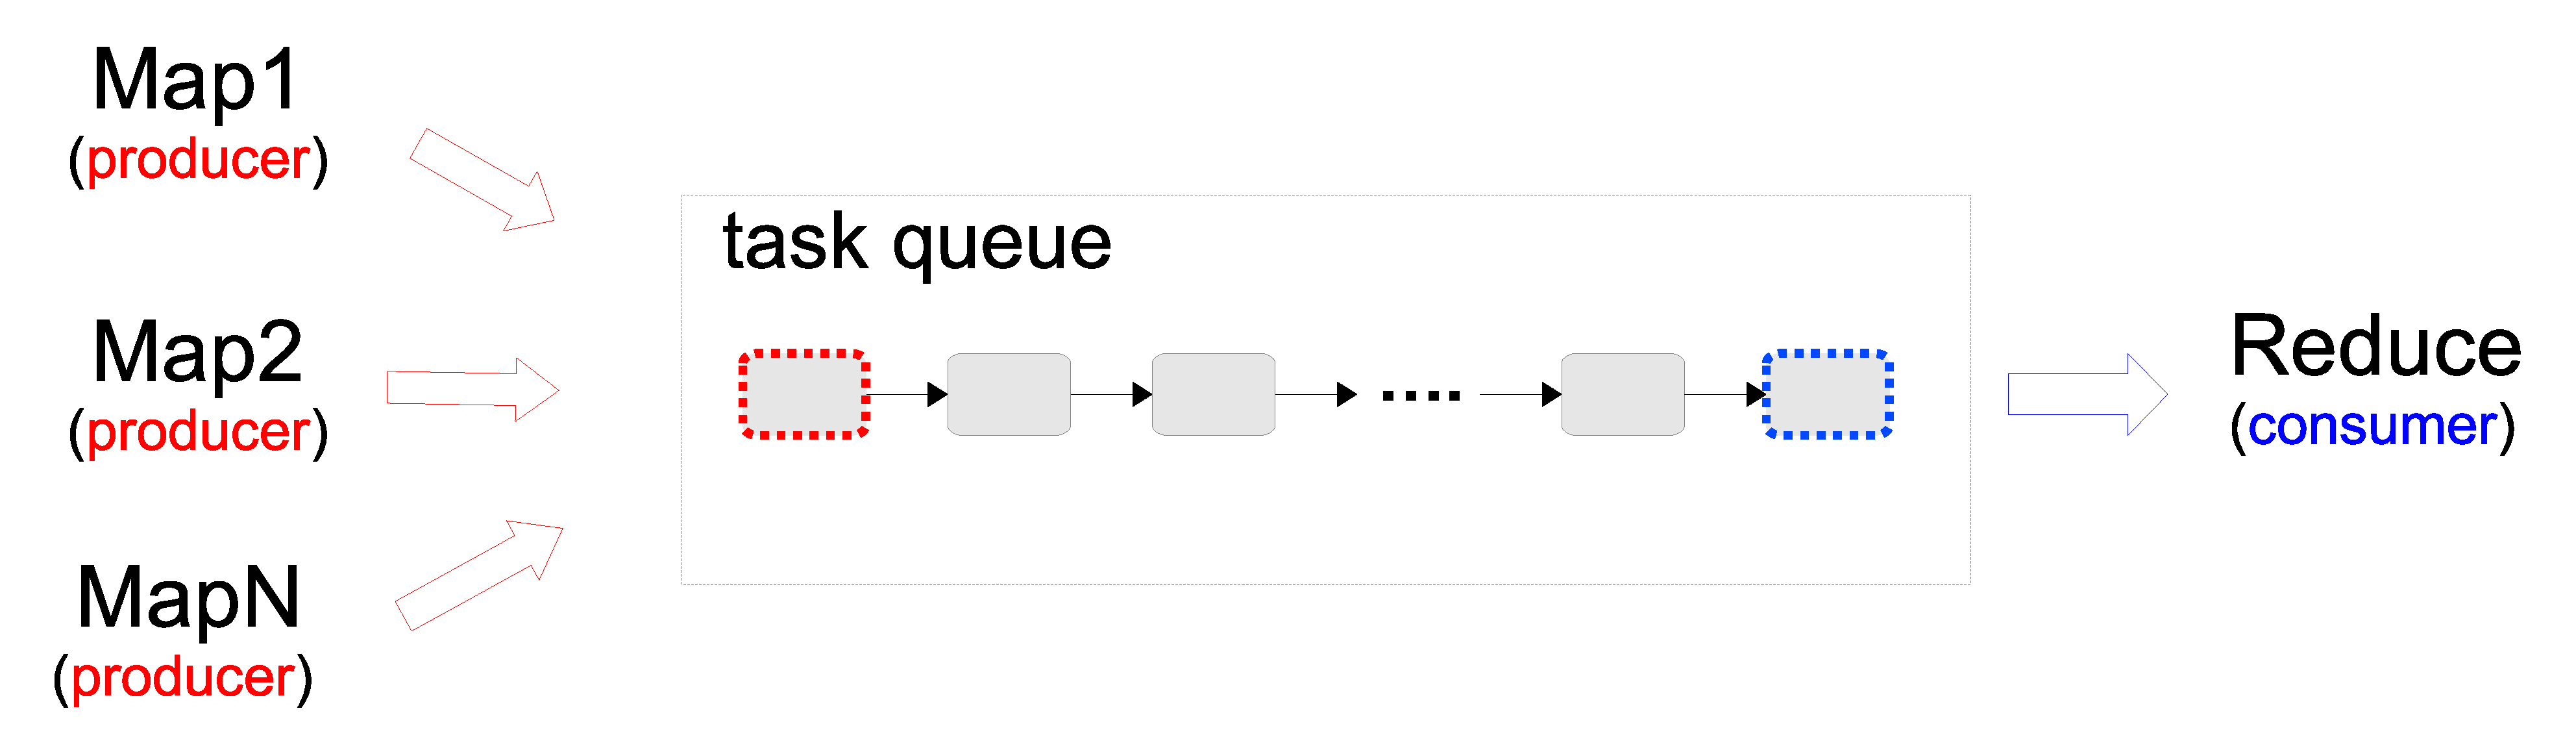
\includegraphics[width=0.5\textwidth]{img/mrphi_pc_model.eps}
    \caption{producer-consumer model in MRPhi}
    \label{mrphi:pc-model}
\end{figure}
虽然MRPhi利用该produce-consume模型实现的Map和Reduce阶段的并发执行,
但是它存在以下两个问题:
\begin{itemize}  
  \item map worker将task插入到queue中之前,需要竞争queue的lock。
  并且线程数越多时,等待lock的开销会越大。
  由于多个map worker同时向task queue中插入任务,
  需要一定的同步机制保证插入的正确性,
  这会造成一定的等待开销。
  \item queue的管理问题,虽然MRPhi\cite{lu2013mrphi}中并没有提到,
  具体的queue是如何管理的,但queue的管理不外乎两种:
  (1)采用固定分配的方式:预先分配一块固定大小的空间,之后重复利用,
  但当queue满,map woker需要停止等待,直到reduce将queue中的数据取走。
  (2)采用动态分配:虽然map worker不需要等待,
  但是会存在大量的动态内存分配和回收的开销。
\end{itemize}
  DMR中使用的producer-consumer模型则不同,
  其中map worker和reduce worker使用一种一对一的隐式queue,
  每个map worker只需将task插入到专属的queue中即可。
  因此,多个map worker不需要竞争queue,从而可有效减少锁的开销。
  
  
\begin{figure}[!h!t]  
    \centering
    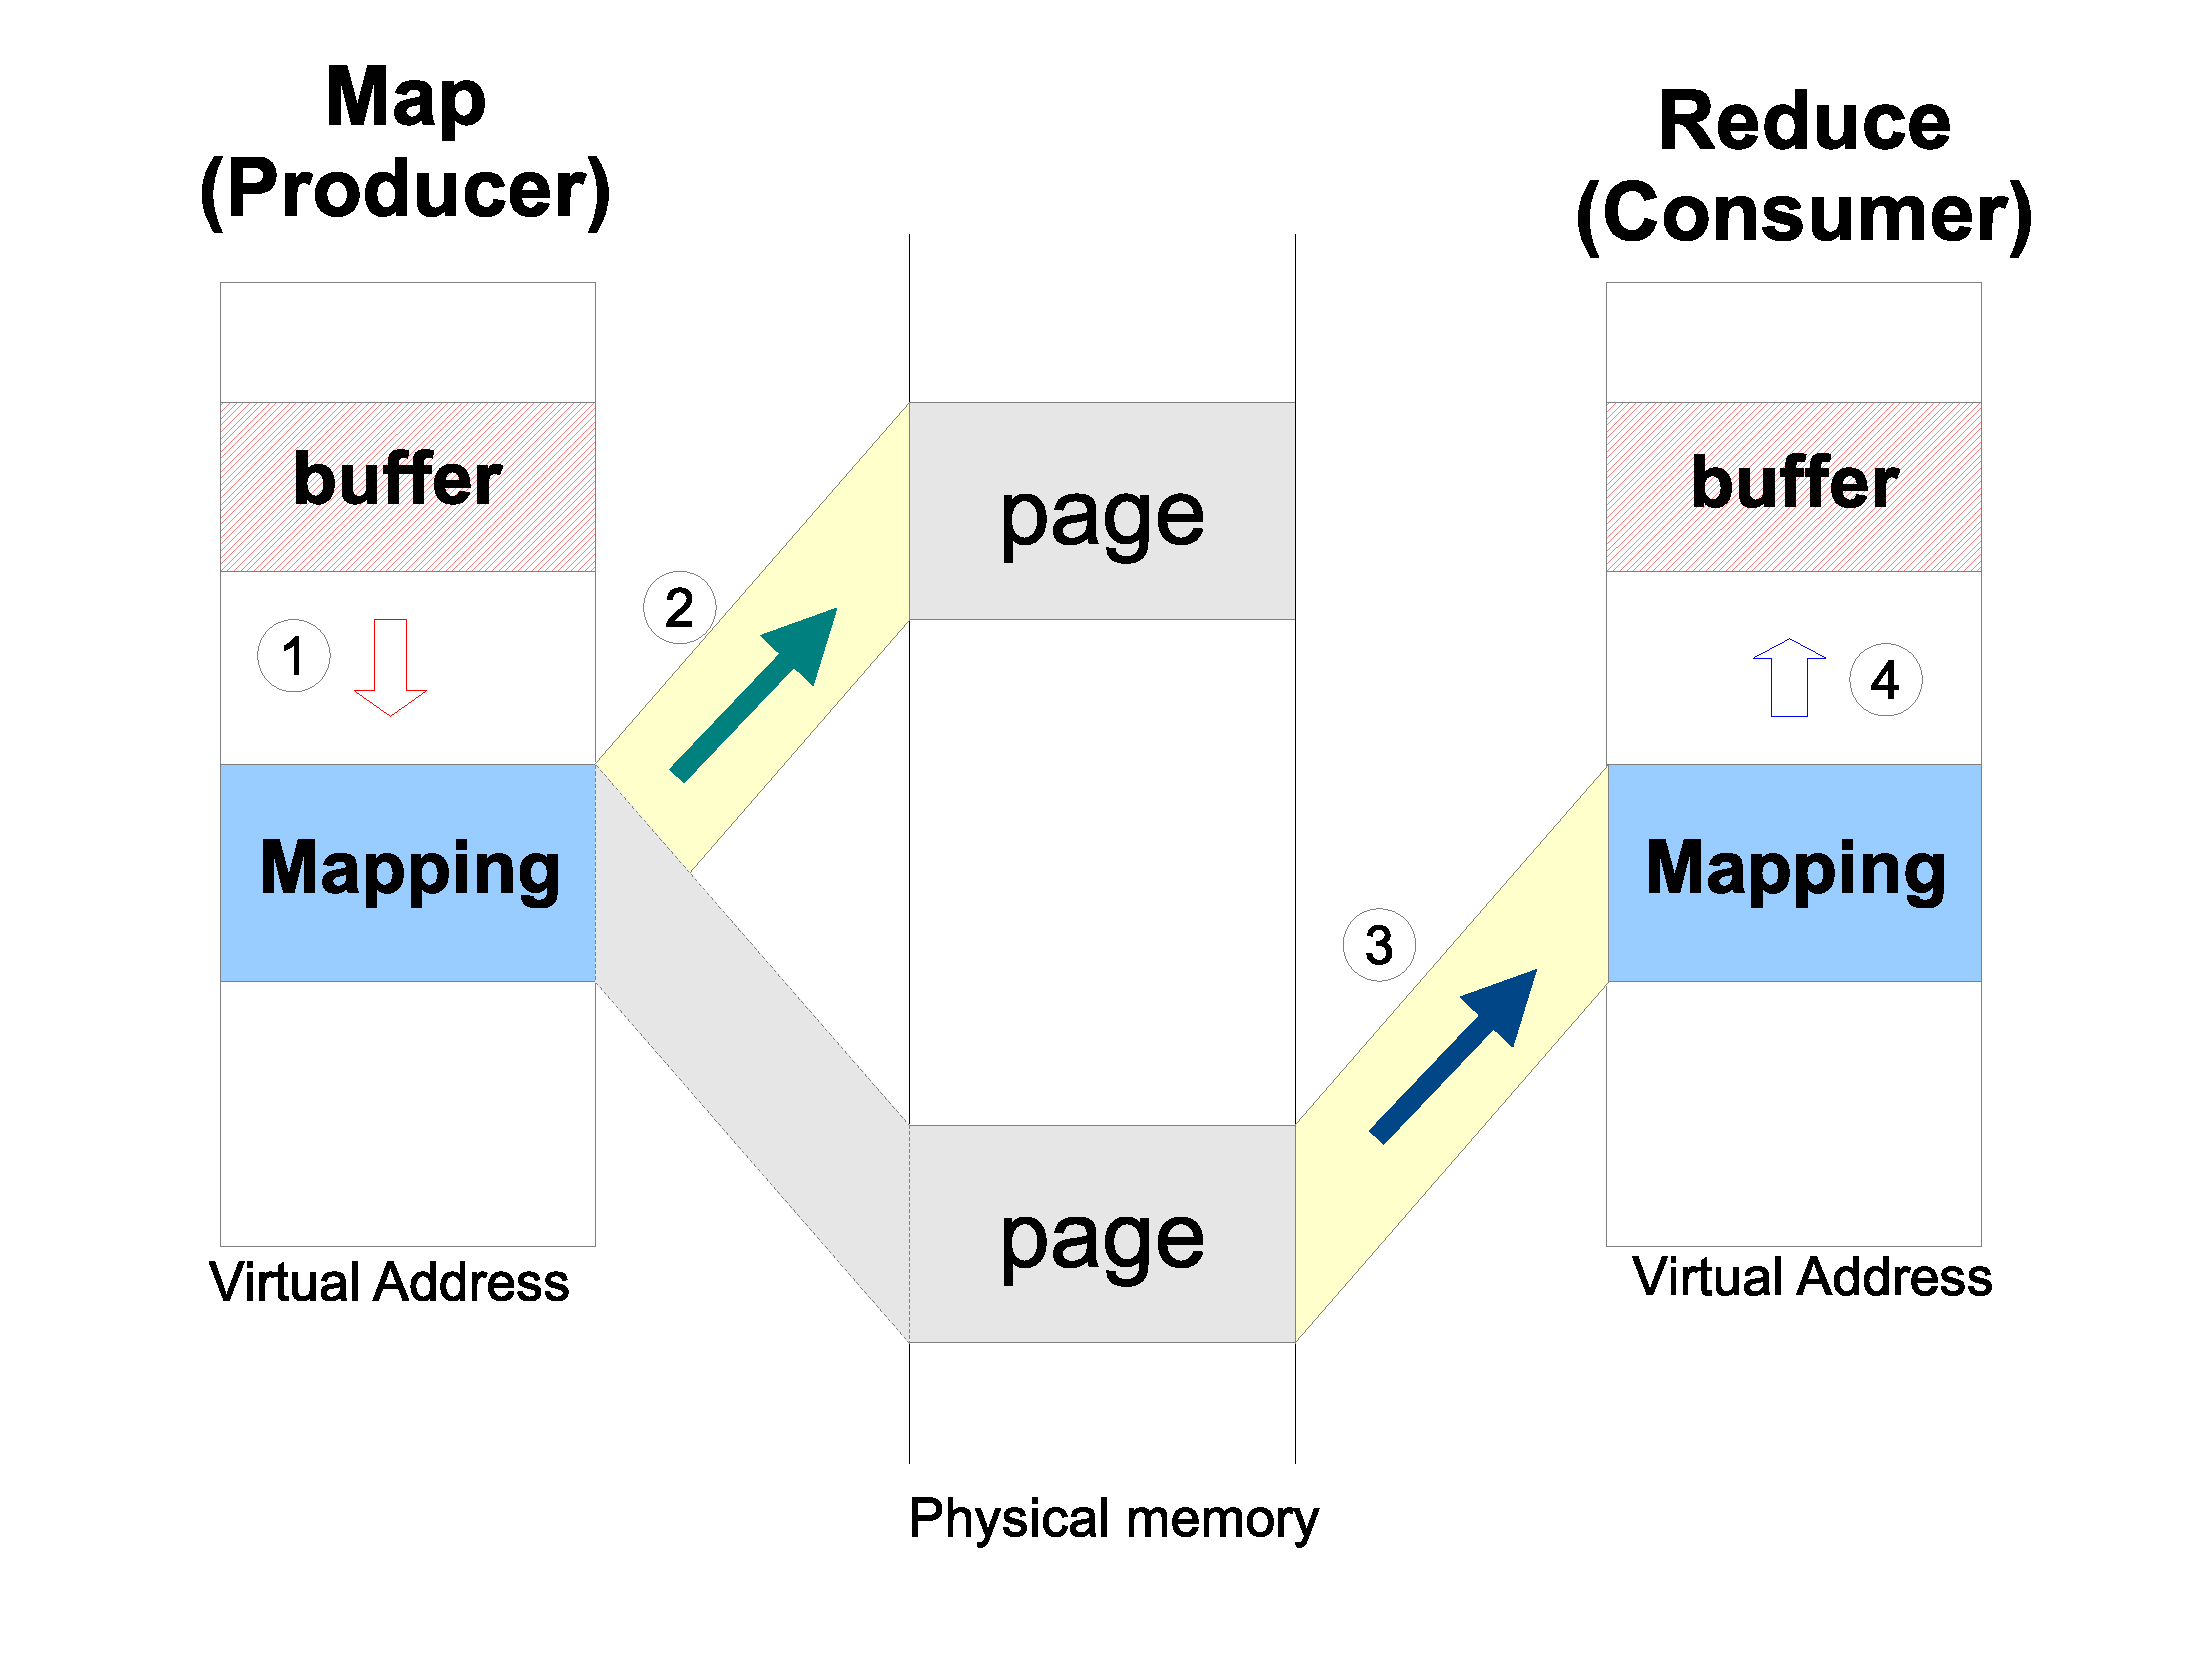
\includegraphics[width=0.5\textwidth]{img/dmr_pc_model.eps}
    \caption{producer-consumer model in DMR}
    \label{dmr:pc-model}
\end{figure}

如图\ref{dmr:pc-model}所示,综上所述,
DMR中producer-consumer模型的关键不同之处有两点:
其一,producer和consumer之间是一对一的隐式queue,
因此producer之间无须竞争,可以避免锁的竞争带来的开销。
其二,producer和consumer之间的隐式queue,
不采用显示的操作,而是采用一种mapping的方式,
即一旦buffer中的数据满,producer便会触发一个send操作,
底层的实现中,会将buffer对应的物理内存加入到隐式queue中,
buffer重新映射到一块新的物理内存,
producer只需将buffer设置为空,
便可继续对buffer进行读写。
这种方式的优点在于其快速高效。

DMR中的具体操作为,map worker向buffer中写入数据,
当buffer满时触发send操作,
之后将buffer标志为空,便可继续向buffer中写数据。
reduce worker以轮循的方式读取各个隐式queue中的数据,
从而,map worker和reduce worker可以并发的进行工作,
且不需要复杂的同步手段。
\input mapbuf
